

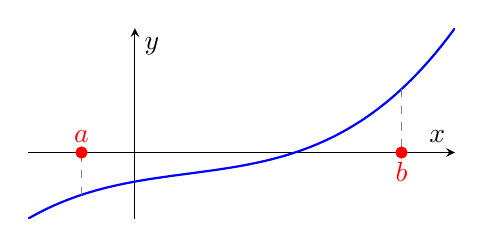
\begin{tikzpicture}
    \begin{axis}[
        axis lines = middle,
        xlabel = $x$,
        ylabel = {$y$},
        xtick = \empty,
        ytick = \empty,
        width=7cm,
        height=4cm
    ]
    
    \addplot[domain=-1:3, samples=100, color=blue, thick]{0.5*(x-.5)^3 + x-2}; % Change this function as per your requirement
    \addplot[mark=*,color=red] coordinates {(-0.5,0)} node[above] {$a$};
    \addplot[mark=*,color=red] coordinates {(2.5,0)}  node[below] {$b$};
    
    \draw [dashed, color=gray] (axis cs: -0.5,-3) -- (axis cs: -0.5,0);
    \draw [dashed, color=gray] (axis cs: 2.5,4.5) -- (axis cs: 2.5,0);
    
    \end{axis}
\end{tikzpicture}
    